\subsection{Glyph: \glyph{Multimer}}
\label{sec:multimer}

As its name implies, a multimer is an aggregation of multiple identical or pseudo-identical entities held together by non-covalent bonds (thus, they are distinguished from polymers by the fact that the later involve covalent bonds).
Here,  \emph{pseudo-identical} refers to the possibility that the entities differ chemically but retain some common global characteristic, such as a structure or function, and so can be considered identical within the context of the SBGN \PD.\borlinghaus{Maybe we should describe pseudo-identical above where we are using it for the first time.}
An example of this is the homologous subunits in a hetero-oligomeric receptor.
\corr{SBGN \PD accepts multimers of \glyph{simple chemical} (\sect{simpleChemical}), \glyph{macromolecule} (\sect{macromolecule}), \glyph{nucleic acid feature} (\sect{genetic}) or \glyph{complex} (\sect{complex}).
}{
SBGN \PD defines four different \glyph{multimer} glyphs: \glyph{simple chemical multimer}, \glyph{macromolecule multimer}, \glyph{nucleic acid feature multimer} and \glyph{complex multimer}.
}
\rougny{Multimer glyphs could also be called \glyph{multimer of simple chemicals}, \glyph{multimer of macromolecules} \dots, the same way as their corresponding SBO terms.}

\begin{glyphDescription}

\glyphSboTerm
\begin{tabular}{l l}
    & SBO:0000286 ! multimer\\
\corr{Simple Chemical}{\glyph{Simple chemical multimer}} & SBO:0000421 ! multimer of simple chemicals\\
\corr{Macromolecule}{\glyph{Macromolecule multimer}} & SBO:0000420 ! multimer of macromolecules \\
\corr{Complex}{\glyph{Complex multimer}} & SBO:0000418 ! multimer of complexes \\
\corr{Nucleic Acid Feature}{\glyph{Nucleic acid feature multimer}} & SBO:0000419 ! multimer of informational molecule segments \\
\end{tabular}

\add{
\glyphIncoming
Zero or more \glyph{production} arcs (\sect{production}).
}

\add{
\glyphOutgoing
Zero or more \glyph{consumption} arcs (\sect{consumption}), \glyph{modulation arcs} (\sect{modulations}), \glyph{logic arcs} (\sect{logicArc}), or \glyph{equivalence arcs} (\sect{equivalenceArc}).
}

\corr{\glyphContainer A \glyph{multimer} is represented by two identical containers shifted horizontally and vertically and stacked one on top of the other, as shown in \fig{multimer}.
The shape of the containers varies depending on the pseudo-identical subunits type (\sect{subunit}).
}{
\glyphContainer
Each \glyph{multimer} is represented by a different shape depending on the bio-molecular nature of its pseudo-identical subunits, as shown in \tab{multimer_containers}.
The shape of a \glyph{multimer} consists of two \corr{\glyph{subunits}/\glyph{EPNs}?}{\glyph{subunits} or \glyph{EPNs}} shapes shifted horizontally and vertically, and stacked on top of another.
}
\rougny{Is this sentence necessary?}

\corr{
\glyphLabel A \glyph{multimer} has no identity on its own\rougny{It is not clearly stated (but suggested) that the label refers to the subunit (should that be? I would say yes. See discussion on sbgn-discuss). I suggest to replace this paragraph by the following one.}\draeger{Let's just stipulate that in cases where people need to label the whole differently from its components that they should not use multimers, but the complex glyph instead.}.  However, the first of the monomers carries an identifying label.  The label is placed in an unbordered box containing a string of characters.  The characters can be distributed on several lines to improve readability, although this is not mandatory.  The label box must be attached to the centre of the top monomer's container.  The label may spill outside of the container.
}{
\glyphLabel
A \glyph{subunit} is identified by a label that is  \corr{an unbordered box containing}{} a string of characters \corr{.
The characters}{that} may be distributed on several lines to improve readability.
% \dogrusoz{again replace "can" with "may" and remove the mandatory part.}
The centre of the label must be placed on the centre of the shape.
The label may extend outside of the shape.
The label should refer to the pseudo-identical subunits, and not to the multimer itself.
}
\rougny{In the map drawn here and there, this is only sometimes the case. Remove the sentence?}

\add{\glyphAux A \glyph{multimer} may carry auxiliary units, depending on its type.}

\add{A \glyph{macromolecule}, \glyph{nucleic acid feature}, or \glyph{complex multimer} can carry one or more \glyph{state variables} that add information about its state (\sect{stateVariable}).
The state of such a \glyph{multimer} is defined as the set of all its \glyph{state variables}.}\blinov{Talking about the state of a multimer is confusing and not necessary.}

\add{A \glyph{multimer} of any type can carry one or more \glyph{units of information} (\sect{unitInfo}).
These can characterize a domain, such as a binding site.
Particular \glyph{units of information} are available for describing the material type (\sect{material-types-cv}), conceptual type (\sect{conceptual-types-cv}) and the cardinality (\sect{cardinality-cv}) of such a \glyph{multimer}}.

\add{Note that a \glyph{state variable} or a \glyph{unit of information} carried by a \glyph{multimer} actually applies to each of the subunits individually.
If instead the \glyph{state variables} or the \glyph{units of information} are meant to apply to the whole multimeric assembly, a \glyph{macromolecule} (\sect{macromolecule}) or a \glyph{complex} (\sect{complex}) should be used instead of a \glyph{multimer}.
An assembly containing some \glyph{state variables} or \glyph{units of information} applicable to the subunits, and other \glyph{state variables} or \glyph{units of information} applicable to the assembly (for instance opening of a channel and phosphorylation of each of its subunits) should be represented by a \glyph{complex} (\sect{complex}).}

\add{Finally, a \glyph{simple chemical multimer} can also carry a \glyph{simple clone marker} (\sect{cloneMarker}), and a \glyph{macromolecule}, \glyph{nucleic acid feature} or \glyph{complex multimer} a \glyph{labelled clone marker} (\sect{cloneMarker}).}

\end{glyphDescription}

\begin{table}[h]
\begin{tabu}{X[c,m]X[c,m]X[c,m]X[c,m]}
    \toprule
    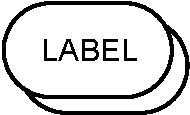
\includegraphics[valign = m]{images/simple_chemical-multimer} & 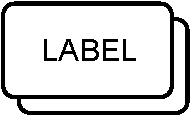
\includegraphics[valign = m]{images/macromolecule-multimer} & 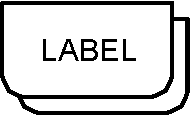
\includegraphics[valign = m]{images/genetic-multimer} & 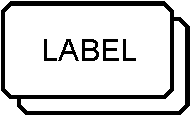
\includegraphics[valign = m]{images/complex-multimer}\\[0.5cm]
    \glyph{simple chemical multimer} & \glyph{macromolecule multimer} & \glyph{nucleic acid feature multimer} & \glyph{complex multimer}\\
	\bottomrule
\end{tabu}
\caption{The \PD glyphs for the different types of \glyph{multimers}.}
\label{tab:multimer_containers}
\end{table}
\toure{Can the 'complex multimer' be lowered in the figure?}
% \begin{figure}[H]
%   \centering
%   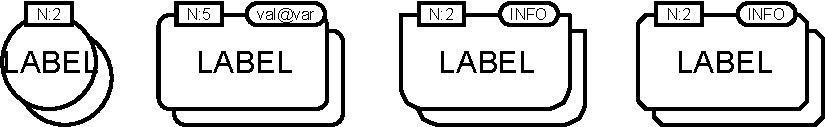
\includegraphics[scale = 0.3]{images/multimer}
%   \caption{The \PD glyph for \glyph{multimer} with an additional unit of information containing the cardinality.}
%   \label{fig:multimer}
% \end{figure}
% \rougny{Add cloned version?}

% The following is for [X]Emacs users.  Please leave in place.
% Local Variables:
% TeX-master: "../sbgn_PD-level1"
% End:
